\documentclass[12pt]{article}
\usepackage[a4paper,margin=2cm]{geometry}
\usepackage{CJKutf8}
\usepackage[utf8]{inputenc}
\usepackage[T1]{fontenc}
\usepackage{listings}
\usepackage{amsmath}
\usepackage{Tabbing}
\usepackage[sorting=none,backend=biber]{biblatex}
%\usepackage[affil-it]{authblk}
\usepackage{lmodern}
\usepackage{titlesec}
\usepackage[skip=2pt,font=footnotesize]{caption}
\usepackage{ulem}
\usepackage{graphicx}

\titlespacing{\paragraph}{\parindent}{0.5em}{0.5em}
\addbibresource{refs.bib}
\renewcommand{\baselinestretch}{1.05}
\lstset{basicstyle=\ttfamily\fontseries{lc}\selectfont,breaklines=true,tabsize=4}

\begin{document}

%\frontmatter
\begin{titlepage}
   \begin{center}

	\large
	\textit{University of Brasília} \\
	
    \vfill
	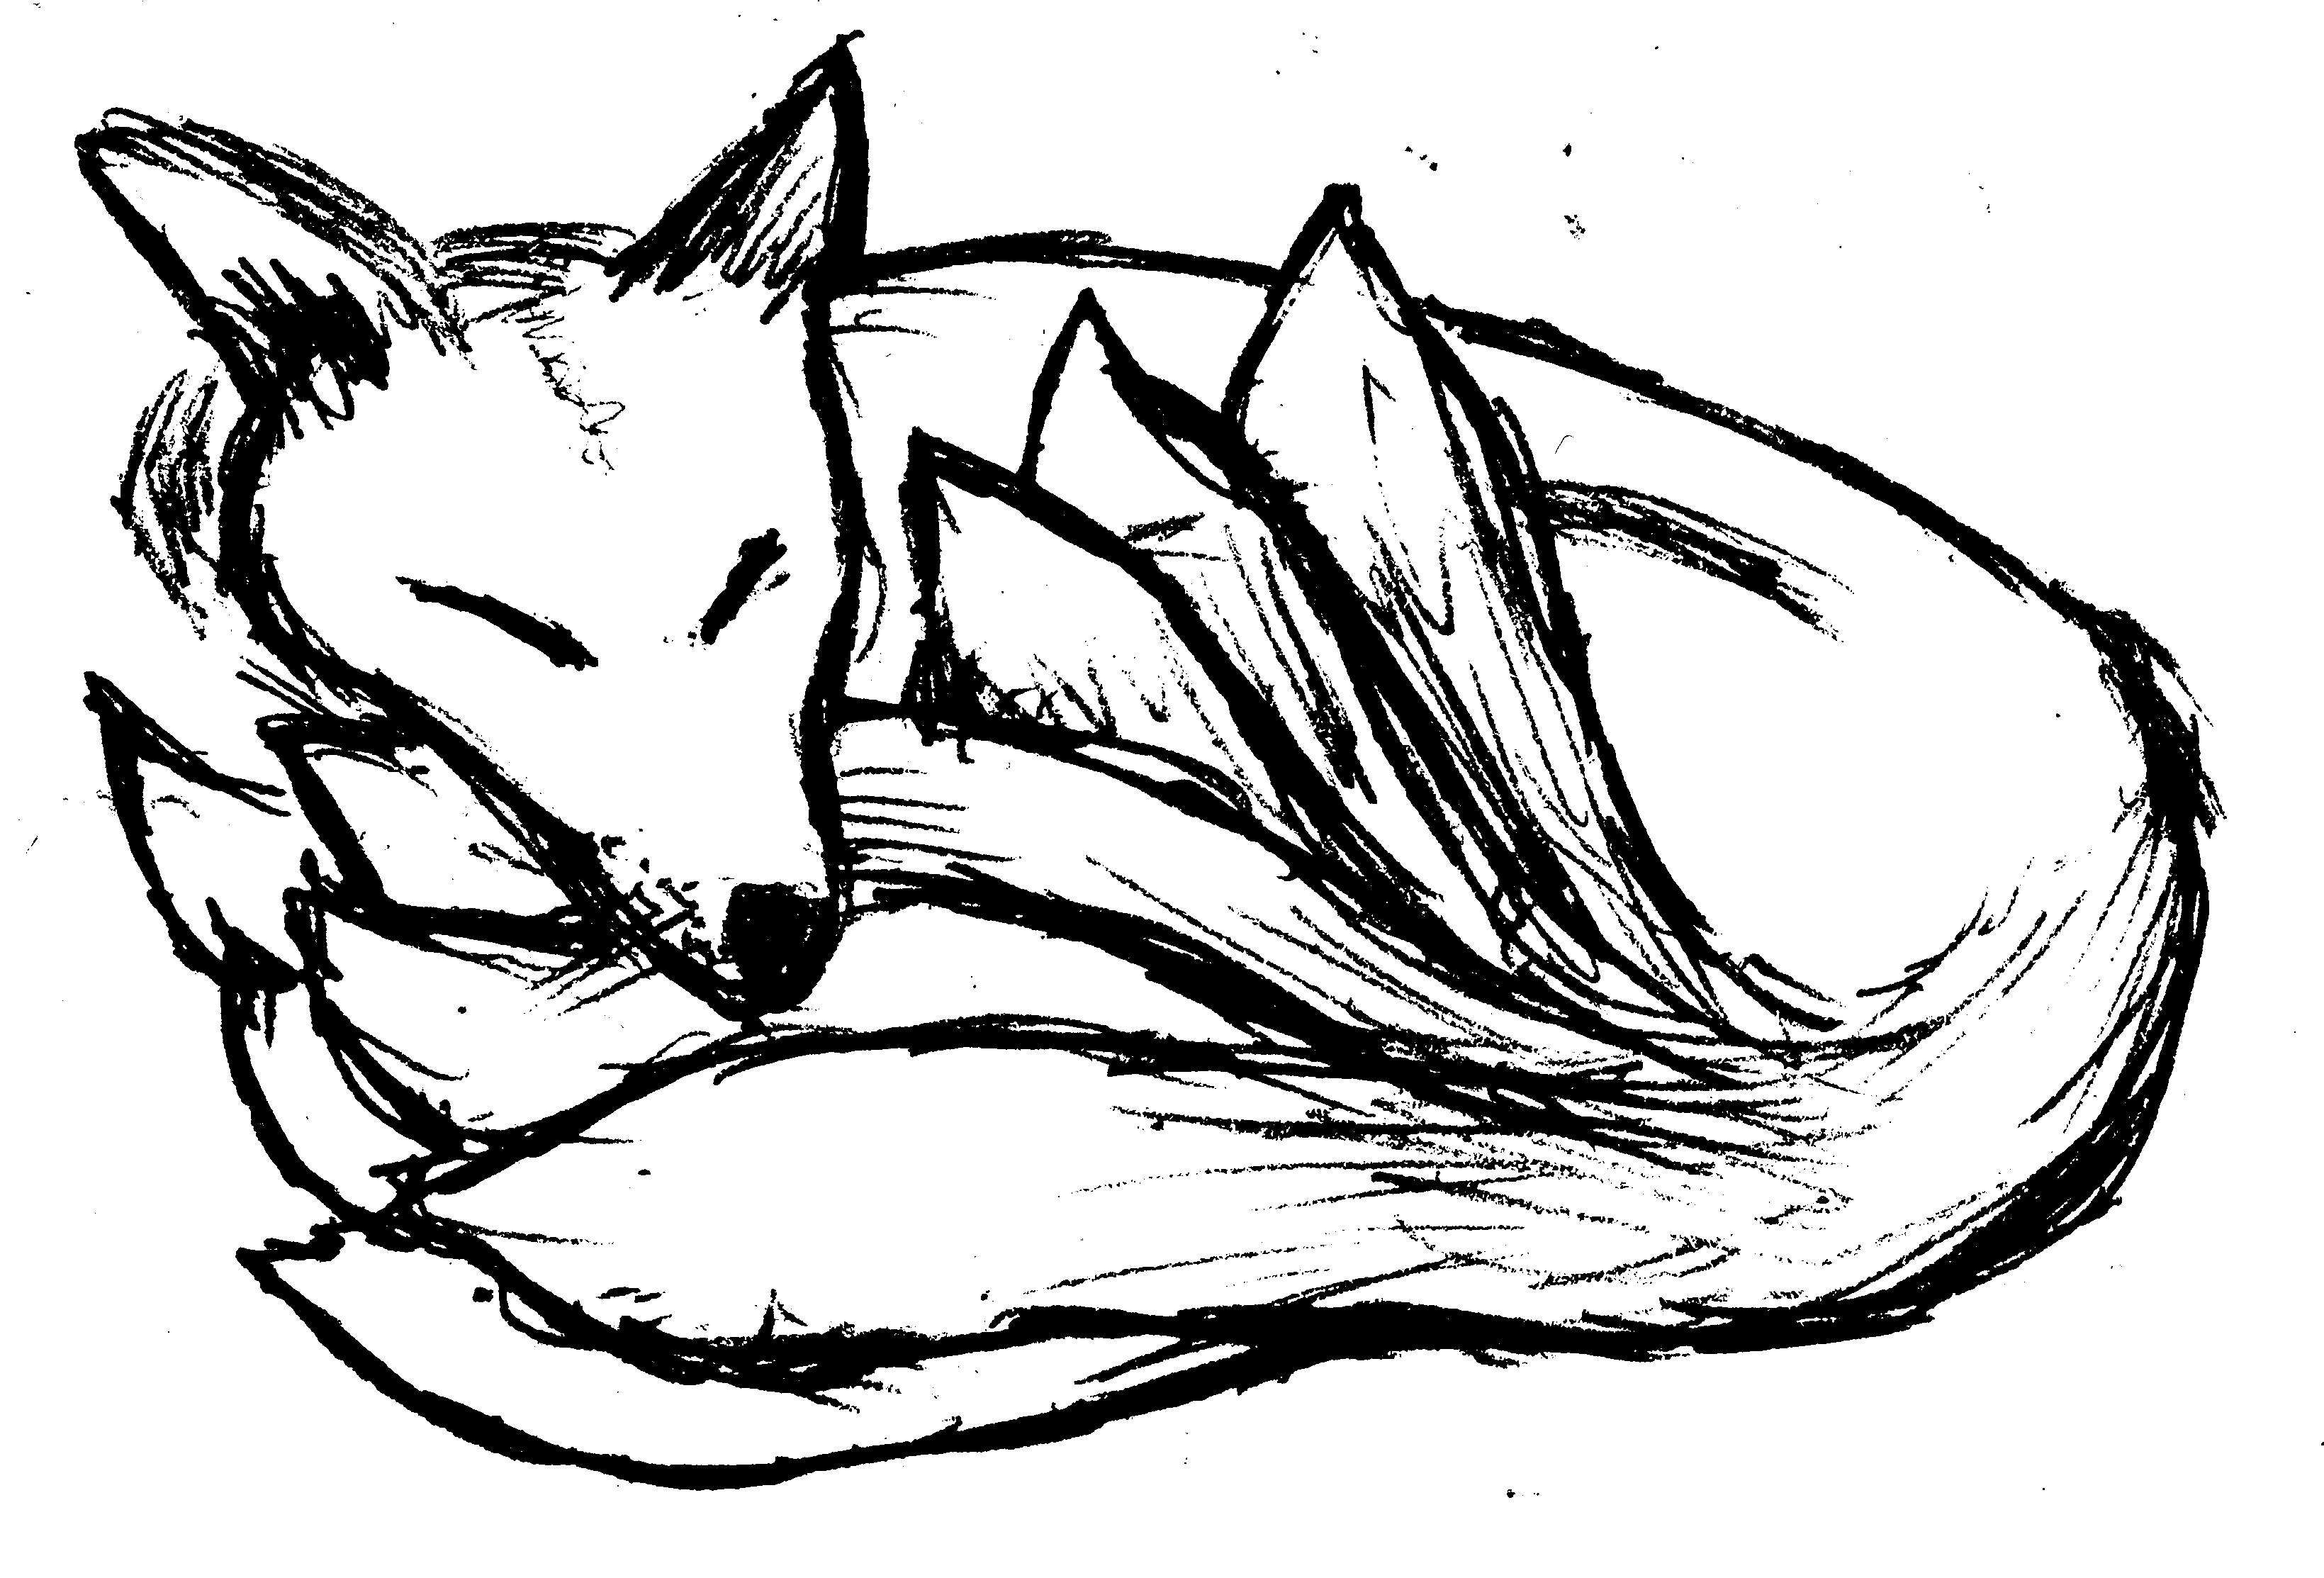
\includegraphics[width=0.27\linewidth]{../slides/kyu.png} \\
	
	\vspace*{0.3cm}
	\small
	\begin{CJK}{UTF8}{min}
		九\hspace{0.57cm}尾\hspace{0.57cm}狐\hspace{0.57cm}の\hspace{0.57cm}語
	\end{CJK} \\
	
	\huge K Language \vspace*{0.3cm} \\
	\normalsize
	Polymorphism in a C-like \\
	programming language \\

	\vspace*{3cm}
	\large
	Diogo César Ferreira\\
	\vspace*{0.3cm}
	11/0027931 \\
	
	\vfill
	\normalsize
	\today
   \end{center}
\end{titlepage}

\clearpage
\tableofcontents

\clearpage
%\mainmatter

% section 1 - introduction
\section{The language}
\subsection{Introduction}
Programming languages are languages that can be converted into sets of instructions to be
executed by a computer. This conversion process is called translation (or compilation) and
is done by software known as compilers. As programming languages evolved, we observe an
increasing variety of abstractions to accommodate for new programming paradigms and
techniques, which also bring them closer to the domain of the problems they are set
out to solve and away from the specificities of architecture set implementations \cite{Aho2007}.

One such abstraction is polymorphism. In typed languages, symbols (named identifiers
for entities such as variables or functions) are constrained by their data type.
If polymorphism is available, we are able to interact with different data types
through a single interface, for instance, by allowing multiple types to be assigned
to a given symbol. Polymorphism improves code readability and helps keeping the namespace
clean by allowing functions to be identified by their expected behavior rather than
contrived by the types of their arguments. Polymorphism is also one of the key features
in object-oriented programming \cite{Aho2007, Strachey2000}.

Aside from the possibility to perform arithmetical operations over a few different
data types (integers, floating point and pointers), the C programming language does
not support polymorphism. In this work we seek to provide polymorphism in the form
of function overloading - where polymorphic functions may have multiple definitions
according to their argument types - to a simplified subset of the C programming language.
The grammar of the language is presented in the following subsection.

 
\subsection{Lexical features}
The following table summarizes what word patterns are part of the language we are designing.
These patterns should be recognized by the scanner, and therefore are provided as an input file
for the FLEX \cite{FLEX} scanner generator (see attached file ``language.l''):

%\paragraph{}
{
\small
%\vfill
\begin{tabular}{lccccccccc}
\textbf{Data types}                      & void & char & int & float &         &      &      &   &   \\
\textbf{Keywords}                        & if   & else & do  & while & return  &      &      &   &   \\
\textbf{Arithmetical operators}          & $+$  & $-$  & $*$ & $/$   & $\%$    & $++$ & $--$ &   &   \\
\textbf{Comparison operators}            & <    & >    & <=  & >=    & ==      & !=   &      &   &   \\
\textbf{Logical operators}               & \&\& & ||   & !   &       &         &      &      &   &   \\
\textbf{Assignment operator}             & =    &      &     &       &         &      &      &   &   \\
\textbf{Character/string delimiters}     & '    & "    &     &       &         &      &      &   &   \\
\textbf{Array indexers}                  & [    & ]    &     &       &         &      &      &   &   \\
\textbf{Scope delims./init lists}        & \{   & \}   &     &       &         &      &      &   &   \\
\textbf{End of statement mark}           & ;    &      &     &       &         &      &      &   &   \\
\textbf{Function args/calls}             & (    & )    &     &       &         &      &      &   &   \\
\textbf{List element separator}          & ,    &      &     &       &         &      &      &   &   \\
\textbf{Comment delimiters}              & /*   & */   & //  &       &         &      &      &   &   \\
\end{tabular}

%\vfill
\vspace{1cm}

\begin{tabular}{ll}
\textbf{Character constants}            & text delimited by single quotation marks (') \\
\textbf{String literals}                & text delimited by double quotation marks (") \\
\textbf{Integer decimal constants}      & e.g. 1, 2, 100, -5, +7                       \\
\textbf{Integer hexadecimal constants}  & e.g. 0x01, -0xA, +0x123                      \\
\textbf{Floating-point constants}       & g.g. 0.0, -1.234, +3.14                      \\
\textbf{Comments and white space}       & are ignored.                                 \\
\end{tabular}
}
 
\subsection{Language syntax}

Our language's grammar contains elements taken from the one presented by \textcite{Harbison2002},
which is a compilation from the many versions of the C grammar specified by the ISO C Standard
along the years. Our grammar follows the general structure of the C language's grammar.
We aim to provide a simplified version of the C language with support for polymorphic function
definitions, that is, which allows the programmer to define multiple functions with the same name
but different argument types. The following grammar is also provided as an input file for the
GNU Bison \cite{BISON} parser generator (see attached file ``language.y'').

\small
\begin{enumerate}
\item \begin{tabbing} declaration-list \= $\rightarrow$ \= declaration \\
	\> \hspace*{0.05cm} | \> declaration-list declaration \\
\end{tabbing}

\item \begin{tabbing} declaration \= $\rightarrow$ \=  function-definition \\
	\> \hspace*{0.05cm} | \> init-declarator \textbf{;} \\
\end{tabbing}

\item \begin{tabbing} init-declarator \= $\rightarrow$ \= var-declarator        \\
	\> \hspace*{0.05cm} | \> var-declarator \textbf{=} assignment-expression    \\
	\> \hspace*{0.05cm} | \> arr-declarator \textbf{=} \textbf{STRING-LITERAL}  \\
\end{tabbing}

\item \begin{tabbing} var-declarator \= $\rightarrow$ \= type \textbf{IDENTIFIER} \end{tabbing}

\item \begin{tabbing} arr-declarator \= $\rightarrow$ \= type \textbf{IDENTIFIER} \textbf{[} \textbf{]} \end{tabbing}

\item \begin{tabbing} function-definition \= $\rightarrow$ \= function-declarator \textbf{\{} statement-list \textbf{\}}   \\
	\> \hspace*{0.05cm} 	|\>  function-declarator \textbf{\{}  \textbf{\}}   \\
\end{tabbing}

\item \begin{tabbing} function-declarator \= $\rightarrow$ \= type \textbf{IDENTIFIER} \textbf{(} argument-list \textbf{)} \\
	\> \hspace*{0.05cm} 	|\>  type \textbf{IDENTIFIER} \textbf{(} \textbf{VOID} \textbf{)}                              \\
\end{tabbing}

\item \begin{tabbing} argument-list \= $\rightarrow$ \= argument \\
	\> \hspace*{0.05cm} | \> argument-list \textbf{,} argument
\end{tabbing}

\item \begin{tabbing} argument \= $\rightarrow$ \= type \textbf{IDENTIFIER} \\
	\> \hspace*{0.05cm} | \> type \textbf{IDENTIFIER} \textbf{[} \textbf{]} \\
\end{tabbing}

\item \begin{tabbing} compound-statement \= $\rightarrow$ \= \textbf{\{} \textbf{\}} \\
	\> \hspace*{0.05cm} | \> \textbf{\{} statement-list \textbf{\}} \\
\end{tabbing}

\item \begin{tabbing} statement-list \= $\rightarrow$ \= statement \\
	\> \hspace*{0.05cm} | \> statement-list statement
\end{tabbing}

\item \begin{tabbing} statement \= $\rightarrow$ \= \textbf{;} \\
	\> \hspace*{0.05cm} | \> init-declarator \textbf{;} \\
	\> \hspace*{0.05cm} | \> assignment-expression \textbf{;} \\
	\> \hspace*{0.05cm} | \> conditional-statement \\
	\> \hspace*{0.05cm} | \> iteration-statement \\
	\> \hspace*{0.05cm} | \> compound-statement \\
	\> \hspace*{0.05cm} | \> return-statement \textbf{;} \\
	\> \hspace*{0.05cm} | \> inline-asm \textbf{;} \\
\end{tabbing}

\item \begin{tabbing} inline-asm \= $\rightarrow$ \= \textbf{ASM} \textbf{(} \textbf{STRING-LITERAL} \textbf{)} \end{tabbing}

\item \begin{tabbing} conditional-statement \= $\rightarrow$ \= if-statement else-statement \end{tabbing}

\item \begin{tabbing} if-statement \= $\rightarrow$ \= \textbf{IF} \textbf{(} assignment-expression \textbf{)} compound-statement \end{tabbing}

\item \begin{tabbing} else-statement \= $\rightarrow$ \= \textbf{ELSE} compound-statement \\
	\> \hspace*{0.05cm} | \> $\varepsilon$ \\
\end{tabbing}

\item \begin{tabbing} iteration-statement \= $\rightarrow$ \= \textbf{WHILE} \textbf{(} assignment-expression \textbf{)} compound-statement \\
	\> \hspace*{0.05cm} | \> \textbf{DO} compound-statement \textbf{WHILE} \textbf{(} assignment-expression \textbf{)} \textbf{;} \\
\end{tabbing}

\item \begin{tabbing} return-statement \= $\rightarrow$ \= \textbf{RETURN} \\
	\> \hspace*{0.05cm} | \> \textbf{RETURN} assignment-expression \\
\end{tabbing}

\item \begin{tabbing} assignment-expression \= $\rightarrow$ \= logical-or-expression \\
	\> \hspace*{0.05cm} | \> postfix-expression \textbf{=} logical-or-expression \\
\end{tabbing}

\item \begin{tabbing} logical-or-expression \= $\rightarrow$ \= logical-and-expression \\
	\> \hspace*{0.05cm} | \> logical-or-expression \textbf{||} logical-and-expression \\
\end{tabbing}

\item \begin{tabbing} logical-and-expression \= $\rightarrow$ \= equality-expression \\
	\> \hspace*{0.05cm} | \> logical-and-expression \textbf{\&\&} equality-expression \\
\end{tabbing}

\item \begin{tabbing} equality-expression \= $\rightarrow$ \= relational-expression \\
	\> \hspace*{0.05cm} | \> equality-expression \textbf{==} relational-expression \\
	\> \hspace*{0.05cm} | \> equality-expression \textbf{!=} relational-expression \\
\end{tabbing}

\item \begin{tabbing} relational-expression \= $\rightarrow$ \= additive-expression \\
	\> \hspace*{0.05cm} | \> relational-expression \textbf{<}   additive-expression \\
	\> \hspace*{0.05cm} | \> relational-expression \textbf{>}   additive-expression \\
	\> \hspace*{0.05cm} | \> relational-expression \textbf{<=} additive-expression \\
	\> \hspace*{0.05cm} | \> relational-expression \textbf{>=} additive-expression \\
\end{tabbing}

\item \begin{tabbing} additive-expression \= $\rightarrow$ \= multiplicative-expression \\
	\> \hspace*{0.05cm} | \> additive-expression \textbf{+} multiplicative-expression \\
	\> \hspace*{0.05cm} | \> additive-expression \textbf{--} multiplicative-expression \\
\end{tabbing}

\item \begin{tabbing} multiplicative-expression \= $\rightarrow$ \= unary-expression \\
	\> \hspace*{0.05cm} | \> multiplicative-expression \textbf{*}   unary-expression \\
	\> \hspace*{0.05cm} | \> multiplicative-expression \textbf{/}   unary-expression \\
	\> \hspace*{0.05cm} | \> multiplicative-expression \textbf{\%}  unary-expression \\
\end{tabbing}

\item \begin{tabbing} unary-expression \= $\rightarrow$ \= postfix-expression \\
	\> \hspace*{0.05cm} | \>  \textbf{!}   unary-expression \\
	\> \hspace*{0.05cm} | \>  \textbf{--}   unary-expression \\
	\> \hspace*{0.05cm} | \>  \textbf{-- --}  unary-expression \\
	\> \hspace*{0.05cm} | \>  \textbf{++}  unary-expression \\
\end{tabbing}

\item \begin{tabbing} postfix-expression \= $\rightarrow$ \= primary-expression \\
	\> \hspace*{0.05cm} | \> \textbf{IDENTIFIER} \textbf{(} \textbf{)} \\
	\> \hspace*{0.05cm} | \> \textbf{IDENTIFIER} \textbf{(} argument-call-list \textbf{)} \\
\end{tabbing}

\item \begin{tabbing} primary-expression \= $\rightarrow$ \= \textbf{IDENTIFIER} \\
	\> \hspace*{0.05cm} | \> \textbf{CONSTANT-INT} \\
	\> \hspace*{0.05cm} | \> \textbf{CONSTANT-HEX} \\
	\> \hspace*{0.05cm} | \> \textbf{CONSTANT-FLOAT} \\
	\> \hspace*{0.05cm} | \> \textbf{CONSTANT-CHAR} \\
	\> \hspace*{0.05cm} | \> \textbf{STRING-LITERAL} \\
	\> \hspace*{0.05cm} | \> \textbf{(} assignment-expression \textbf{)} \\
\end{tabbing}

\item \begin{tabbing} argument-call-list \= $\rightarrow$ \= assignment-expression \\
	\> \hspace*{0.05cm} | \> argument-call-list \textbf{,} assignment-expression
\end{tabbing}

\item \begin{tabbing} type \= $\rightarrow$ \= \textbf{VOID} \\
	\> \hspace*{0.05cm} | \> \textbf{INT} \\
	\> \hspace*{0.05cm} | \> \textbf{FLOAT} \\
	\> \hspace*{0.05cm} | \> \textbf{CHAR}
\end{tabbing}

\end{enumerate}
\normalsize

\subsubsection{Grammar changes}
\paragraph{Rule 1:} \textit{declaration-list} is the start symbol once more. We now use Bison's \texttt{\%destructor}
to capture the syntax tree's root.

\paragraph{Rules 3, 4 and 5:} the \textit{init-declarator} has been broken down into rules 4 and 5 to avoid
the need to write many possible combinations of variables in these rules. Initializer lists were removed
from this because integer and float arrays have not yet been implemented (the only implemented arrays are strings).
%Previous version:
%\begin{tabbing} init-declarator \= $\rightarrow$ \= type \textbf{IDENTIFIER}                                                                \\
%	\> \hspace*{0.05cm} | \> type \textbf{IDENTIFIER} \textbf{=} assignment-expression                                                      \\
%	\> \hspace*{0.05cm} | \> type \textbf{IDENTIFIER} \textbf{[} assignment-expression \textbf{]}                                           \\
%	\> \hspace*{0.05cm} | \> type \textbf{IDENTIFIER} \textbf{[} \textbf{]} \textbf{=} \textbf{\{} initializer-list \textbf{\}}             \\
%	\> \hspace*{0.05cm} | \> type \textbf{IDENTIFIER} \textbf{[} \textbf{]} \textbf{=} \textbf{\{} initializer-list \textbf{,} \textbf{\}}  \\
%	\> \hspace*{0.05cm} | \> type \textbf{IDENTIFIER} \textbf{[} \textbf{]} \textbf{=} \textbf{STRING-LITERAL}                              \\
%\end{tabbing}


\paragraph{Rules 6 and 7:} \textit{function-definition} was broken down into rules
6 and 7 to avoid the need to write many possible combinations of variables in these rules.
Function without arguments now need to be declared with ``void'' as the sole argument.
%Previous version:

%\begin{tabbing} function-definition \= $\rightarrow$ \= type \textbf{IDENTIFIER} \textbf{(} argument-list \textbf{)} \textbf{\{} statement-list \textbf{\}}   \\
%	\> \hspace*{0.05cm} 	|\>  type \textbf{IDENTIFIER} \textbf{(} \textbf{VOID} \textbf{)}          \textbf{\{} statement-list \textbf{\}}   \\
%	\> \hspace*{0.05cm} 	|\>  type \textbf{IDENTIFIER} \textbf{(} \textbf{)}               \textbf{\{} statement-list \textbf{\}}   \\
%	\> \hspace*{0.05cm} 	|\>  type \textbf{IDENTIFIER} \textbf{(} argument-list \textbf{)} \textbf{\{}                \textbf{\}}   \\
%	\> \hspace*{0.05cm} 	|\>  type \textbf{IDENTIFIER} \textbf{(} \textbf{VOID} \textbf{)}          \textbf{\{}                \textbf{\}}   \\
%	\> \hspace*{0.05cm} 	|\>  type \textbf{IDENTIFIER} \textbf{(} \textbf{)}               \textbf{\{}                \textbf{\}}   \\
%\end{tabbing}

\paragraph{Rules 12 and 13:} new statement \textit{inline-asm} (rule 13) was created and
included in the list of possible \textit{statement}s (rule 12). That new rule allows for
direct translation of string literals into the generated code (see Section \ref{section:codegen}).

\paragraph{Rules 14, 15 and 16:} \textit{conditional-statement} has been broken down into its
\textit{if-statement} and \textit{else-statement} counterparts. This was done to resolve a
reduce/reduce type conflict that would arise due to a mid-rule action. The \textit{else-statement}
also produces the empty string ($\varepsilon$), so that it is still possible to use an \textit{if}
without an \textit{else}.
%Previous version:

%\begin{tabbing} conditional-statement \= $\rightarrow$ \= \textbf{IF} \textbf{(} assignment-expression \textbf{)} compound-statement \\
%	\> \hspace*{0.05cm} | \> \textbf{IF} \textbf{(} assignment-expression \textbf{)} compound-statement \textbf{ELSE} compound-statement \\
%\end{tabbing}

\paragraph{Rule 27:} postfix array indexing operator has been left out from this version since
array indexing are not yet implemented.
%Removed production:
%\begin{tabbing} postfix-expression \= $\rightarrow$ \= \textbf{IDENTIFIER} \textbf{[} assignment-expression \textbf{]} \end{tabbing}

\subsubsection{Input / output}
Input and output operations are not specified in our language's grammar. However, these are be provided
in the form of a small standard I/O library composed of special polymorphic functions which are always
available to the user. The available functions have the following signatures:

\begin{lstlisting}[language=C]
void write(int i){...}    // outputs an integer to the standard output
void write(char c){...}   // outputs a character to the standard output
void write(char[] s){...} // outputs a string to the standard output
void write(float f){...}  // outputs a float to the standard output
void write(void){...}     // outputs a new line to the standard output

int read(int i){...}     // reads an integer from the standard input and returns it
char read(char c){...}   // reads a character from the standard input and returns it
float read(float f){...} // reads a float from the standard input and returns it
\end{lstlisting}

The \texttt{write} functions output the value provided to them as argument. They do not
otherwise modify the provided value. Example use:

\begin{lstlisting}[language=C]
// output 3 to the standard output
write(3);
\end{lstlisting}

Since there are no pointers in the language, the \texttt{read} functions require an argument
in order to resolve which data type will be read and returned (that is, which function
will be used to read from the standard input). However they do not in any way use or modify the
provided argument. Example use:

\begin{lstlisting}[language=C]
// read an integer from the standard input and
// store it in variable a. The value of a is
// not used within the function read.
int a = read(a);
\end{lstlisting}

As with any other function, \texttt{read} and \texttt{write} are polymorphic and the users are
allowed to define their own versions of these functions, provided that they do not have the same parameters
as the ones already defined. We simulate linking of the library to user code by creating a temporary file
in which the library is concatenated with the input file.

 
\subsection{Semantics}
\label{section:semantics}

\subsubsection{Scope}

Except in the case of initializer lists, scopes are enclosed by curly
braces ('\{' and '\}'). Every program should have at least one scope,
which is the global scope, where the programmer is only allowed to
declare and initialize (but not assign) global variables and to
define functions. Functions can be defined only in the global scope.

The body of a function is treated as a compound statement itself 
and compound statements can be nested. Within compound statements,
there can be variable declaration, initialization and assignment,
arithmetic and logical expressions, flow control statements
(conditional and loops) and jump statements (return).
Since variable assignment can only be done within compound statements
and these are not allowed in the global scope, then a program must
have at least one function for variables to be able to be assigned.
Variables and functions must always be declared, initialized or defined 
before they can be used.

Declaration of variables with the same name in a given scope is
not allowed. However, a variable declaration is allowed to shadow
another variable in a parent scope. When a variable must be used,
a declaration of that variable will be first searched in the
in the current scope. If not found, it will be searched in the
current scope's parent scope and so forth up to the global scope.

Unlike in the C programming language, definition of functions with
the same name is allowed, provided that the functions have different
argument types. Definition of functions with the same name and same
argument types is not allowed, even if the return type differs.
The argument variable names pertain to the outermost scope enclosed
by the function's body.



\subsubsection{Implicit type conversion}
\label{section:types}

Our language is comprised of five basic types:
\texttt{void} (no type), 
\texttt{char} (characters),
\texttt{int} (integers),
\texttt{float} (floating point numbers),
and pointers in the form of arrays of one of the basic types:
\texttt{char[]} (strings),
\texttt{int[]} (arrays of integers),
\texttt{float[]} (arrays of floating point numbers). Notice however, that among the array types,
only strings have been implemented in this version (see Section \ref{section:codegen}).
The rules for conversions are as follows:

\begin{itemize}
 \item \textbf{Same type} when values are of the same type, no conversion is needed;
 \item \textbf{\texttt{void}} cannot be implicitly converted to another type;
 \item \textbf{\texttt{char}} can be implicitly converted to \textbf{\texttt{int}} or \textbf{\texttt{float}};
 \item \textbf{\texttt{int}} can only be implicitly converted to \textbf{\texttt{float}};
 \item \textbf{\texttt{float}} cannot be implicitly converted to another type;
 \item \textbf{Arrays} cannot be implicitly converted to another type.
\end{itemize}

Essentially, a value can be implicitly converted to another type with larger storage size.
For function calls, the same rules should apply after the function's return value has been
resolved. However, types are not implicitly converted on the arguments of a function call.

\subsubsection{Explicit type conversion}

Since there are no casts in the language, there can be no explicit type conversion.

\subsubsection{Expressions and static evaluation}

Most of the language's operators are left-associative with the exception of unary operators
and the assignment operator, which are right-associative. Expressions are first type checked
for incompatibilities. If no type errors are found and the expressions
are composed only of constants, then they will be statically evaluated.


 
\subsection{Use-cases}
We present some use cases in which polymorphic functions would be useful. Functions with the same behavior, but different argument types:

\begin{lstlisting}[language=C]
int   i = -1;
float f = -1.0;
abs(i); // return the absolute value of i
abs(f); // return the absolute value of f
        // In C, abs does not accept a floating-point argument
        // we must use fabs instead
\end{lstlisting}

In this simple example, the abs function could compute the absolute of any numeric value passed as argument. The type constrains in C, however, do not allow the abs function to be called with a floating-point argument.

Functions with different behavior, but the same "intuitive meaning" for the programmer

\begin{lstlisting}[language=C]
int  i[3] = { 9, 2, 5 };
char w[][9] = { "word", "vocable", "locution" };

sort(i); // The user implements a sorting function for integer vectors
sort(w); // The user implements a lexicographic or alphabetic
         // sorting function for string vectors
\end{lstlisting}

The implementation of a sorting function for integers and strings would be considerably distinct. However, intuitively a programmer might expect some notion of ordering to be present in arrays of strings. This can also be applied to functions with different number of arguments:

\begin{lstlisting}[language=C]
// Should return the lowest of either x or y
int min(int x, int y) {
	if (x <= y) { return x; }
	else { return y; }
}

// Should also return the lowest of either x, y or z
int min(int x, int y, int z) {
	if (x <= y) {
		if (x <= z) { return x; }
		else { return z; }
	} else {
		if (y <= z) { return y; }
		else { return z; }
	}
}
\end{lstlisting}

 
%\clearpage

% section 2 - the compiler
\section{The compiler}
In this section we will describe the compiler's implementation for the K Programming Language,
which has the responsibility to read the input text and ultimately convert it into an
executable file. The first step is to define the patterns which are to be recognized by the scanner.
Then, the Fast Lexical Analyzer (FLEX) \cite{FLEX} software is used to generate the lexical
analyzer's main functionality. Moreover we provide the language's grammar to the GNU Bison parser
generator \cite{BISON} which generates the syntax analyzer. Additional routines for input, output,
error handling and data structures to build the syntax tree and symbol table were also implemented
and will be explained in detail later.


\subsection{Program usage}
The program takes one argument which should be a path to the input file.

\begin{lstlisting}
$ ./a.out <input_file>
\end{lstlisting}

The program will then output the symbol table along with the
annotated syntax tree generated from the input file, if it is part of the language.
Should there be errors, the program will instead list them along with their
positions in the text (line and column numbers, where tabs count as 4 columns).

\subsubsection{Compilation instructions}

\begin{enumerate}
\item (Optional) Generate the lexical analyzer .c source code through FLEX
\begin{lstlisting}
$ flex language.l
\end{lstlisting}

\item (Optional) Generate the syntax analyzer .c source code through GNU Bison
\begin{lstlisting}
$ bison -Wall language.y
\end{lstlisting}

\item Compile the program
\begin{lstlisting}
$ gcc -std=c18 -m64 -O3 src/main.c src/node.c src/node-list.c src/table.c src/table-stack.c src/arg-list.c src/parser.c src/scanner.c
\end{lstlisting}

\item Alternatively, a makefile has also been provided which will run all commands
\begin{lstlisting}
$ make
OR
$ make flex   # for step 1
$ make bison  # for step 2
$ make rel    # for step 3
\end{lstlisting}
\end{enumerate}

\paragraph{Technical specifications}
\paragraph{Operating system:} Debian GNU/Linux bullseye/sid (testing release)
\paragraph{Compiler version:} gcc (Debian 9.2.1-17) 9.2.1 20191102
\paragraph{FLEX version:} flex 2.6.4
\paragraph{GNU Bison version:} bison (GNU Bison) 3.4.2

\subsubsection{Attached files}
\begin{lstlisting}
a.out       - Precompiled x64 binary
language.l  - FLEX definitions file
language.y  - BISON definitions file
makefile    - 
src/        - Source code folder
tests/      - Test input files
\end{lstlisting}



\subsection{The symbol table}
We use a single hash table with linked lists as buckets, defined in \texttt{table.h} and
\texttt{table.c}, to implement the symbol table. If performance becomes an issue due to high
load factor, the table can be rehashed to decrease its load factor. Each entry in the symbol
table is comprised of a key and its attributes. The following attributes are currently being
stored:

\begin{itemize}
 \item \textbf{Symbol type}: indicates if the symbol is a variable, a function or some other abstract
 structure such as a scope enclosed by a compound statement;
 \item \textbf{Return type}: stores a function's return type or a variable's data type;
 \item \textbf{Value}: an union that stores a symbol's current value, if applicable;
 \item \textbf{Argument list}: a structure that stores a function's argument list, if there is one;
 \item \textbf{Pointer to node}: a pointer to a node in the syntax tree that represents a statement's body
 \item \textbf{Scope}: a pointer to this symbol's enclosing scope, which itself is an entry in
 some other symbol table.
\end{itemize}

As per current implementation, the data structure used for a symbol table is the same
data structure used for a symbol itself. Therefore, each entry in the symbol table is also a
symbol table. The reason for this is to make the implementation of some auxiliary data structures
simpler: there would be a pointer to a new symbol table in the attributes of a symbol anyway, since
some entries such as functions and compound statements have their own child scope.

\subsubsection{Polymorphic functions}

Whereas variables are included into the table based solely on their names, the insertion of
a function in the table uses a two-step hashing scheme: first, the function is hashed by its
name and inserted into the table. This symbol is now a new symbol table itself.
A key that represents the function's argument types is then constructed from its argument list,
hashed and inserted into this new symbol table. Again, this symbol is another symbol table,
which now holds the scope of the function's body, where the argument variable names are added
to. For example, the following code:

\begin{lstlisting}
int min(int x, int y) {}
int min(int x, int y, int z) {}
\end{lstlisting}

Would generate the following entries in the symbol table:

\begin{lstlisting}
min  <s_type=FUNCTION,r_type=int,args=void>                   # function name
   int,int  <s_type=FUNCTION,r_type=int,args=int,int>         # arg types for min(int,int)
      x  <s_type=VARIABLE,r_type=int,args=void>               # arg 1 of min(int,int)
      y  <s_type=VARIABLE,r_type=int,args=void>               # arg 2 of min(int,int)
   int,int,int  <s_type=FUNCTION,r_type=int,args=int,int,int> # arg types for min(int,int,int)
      x  <s_type=VARIABLE,r_type=int,args=void>               # arg 1 of min(int,int,int)
      y  <s_type=VARIABLE,r_type=int,args=void>               # arg 2 of min(int,int,int)
      z  <s_type=VARIABLE,r_type=int,args=void>               # arg 3 of min(int,int,int)
\end{lstlisting}


Thus, a function call would look up for a function in the current scope's symbol table,
then builds the argument types key from the types resolved by the type checker and looks
up for such an entry in the function's symbol table. In the present version, the type checker
is unable to determine the types of function calls. However, insertions and redefinition
errors are being correctly handled.

\subsubsection{Scope resolution}

The symbol table is also responsible for scope resolution issues. Whenever a variable declaration
is found, the analyzer looks up for its name in the current scope. If it is found, a symbol
re-declaration error is thrown, otherwise, the variable is added to the current scope's table.
Whenever a variable is used, the analyzer looks up for its name in the current scope. If it is
not found, the analyzer searches the parent scope and then its parent all the way up to the global
scope or until a declaration is found. If none is found, an undeclared variable error is thrown.

\subsubsection{Scope management}

Scopes are stored withing a stack structures which elements are symbol tables. The stack
is initialized with a single element that corresponds to the program's global scope.
Whenever the parser finds a rule that would begin a new scope, then a new symbol, with an
appropriately given key is inserted into the current context (top of the stack) and then
pushed onto the stack, becoming the new element on the top, thus the new current
context. When the parser finds the terminal token that ends a scope the parser pops
the context from the stack, leaving its parent on the top.
These actions are handled by the parser and are defined in the GNU Bison input file in
rules such as this:

\begin{lstlisting}
 compound_statement
	: ...
	| '{'    { begin(NULL); }    statement_list '}'    { $$ = $3  ; finish(); }
\end{lstlisting}

Here, \texttt{begin(NULL)} is a mid-rule action whose only purpose is to create a new context
and push it to the stack and \texttt{finish()} pops the stack when the context is closed.










\subsection{Syntax tree}
To build the syntax tree, we use the data structures defined in \texttt{node.h} and \texttt{node.c}.
By setting Bison's default data type a pointer to our tree node type, we are now able to start
building our syntax tree as the parser proceeds.
\begin{lstlisting}
%union {
	struct node * node;
}
\end{lstlisting}

The scanner transforms some terminal tokens into leaf nodes for the tree. The structures
are allocated and then passed to the parser via the \texttt{yylval} variable:

\begin{lstlisting}[caption={Example of a lexer rule where a leaf node is created.
This procedure is preformed for
all data types, identifiers and constants.},captionpos=b]
"int"	{
			update_position();
			int t = INT;
			yylval.node = node_init(node_list, t, yytext, NULL);
			return t;
		}
\end{lstlisting}

Then, the parser is instructed to connect these nodes forming the syntax tree.
Nodes are connected for most (except when the \texttt{error} token is present)
grammar productions. In some cases, such as when an identifier is found, a symbol is also added
to the symbol table.

\begin{lstlisting}[caption={Example of a parser rule where nodes are connected.
This procedure is preformed for all productions, except error handlers. Here, a symbol
is also added to the symbol table through the function \texttt{add\_symbol\_var}},captionpos=b]
declarator : type IDENTIFIER 
	{
		$$ = node_init(node_list, 'D', "declarator-variable", $1, $2, NULL);
		add_symbol_var($$);
	}
\end{lstlisting}

\subsection{Type checker}
\label{section:tc}

Every time the parser performs a reduction for a statement rule and
creates a node in the tree, it is also type-checked
(See Listing \ref{lst:newnode} for example).
Type-checking is performed by the functions declared
in the header ``typechecker.h'', and it is responsible
for the following actions:

\begin{enumerate}
 \item Verify whether operations and operands have compatible types;
 \item If possible, perform static evaluation: if all operands in an expression are constants, evaluate it;
 \item If not possible to perform static evaluation, genereate the corresponding code;
\end{enumerate}

The rules for type convertion during either static evaluation
or code generation are the same as the ones presented in Section
\ref{section:types}:
\texttt{char} can be promoted to \texttt{int},
\texttt{int} can be promoted to \texttt{float} and other types cannot
be part of expressions. In the middle of expressions, if either operand
is able to be promoted it will be so. Therefore, unless the user tries
to perform an operation with a \texttt{void} type or array, type errors
will only be reported on assignments and function calls (arguments of
function calls are never converted).


The type checker links the node it just analyzed to an entry in the symbol table,
setting its attributes accordingly. However, in order to release resources,
the type checker also prunes a node's children from the tree after it has been successfuly analyzed,
because we no longer requre the data held by the children at this point: either they have
been statically evaluated or the corresponding code has already been generated.

\subsection{Static evaluation}

Static evaluation is performed by the functions expanded from the
preprocessor macros defined in the header ``evaluator.h''. These
macros define the expected behavior and appropriate type convertions
for each arithmetic, logical and relational operators present in the
language. The evaluator also sets flags for type errors that still
may occur inside expressions, such as operations with \texttt{void} or
arrays.

The program uses an internal operation stack for static evaluation.
The operands are popped from the stack and, if both are constans,
the operation is evaluated and the result is pushed back into the
stack, which will then be available for the next time the parser
reduces a rule and calls the type checker again.

\subsection{Code generation}

\subsection{Error handling}
As the program reads the input file, the parser requests tokens from the scanner, who splits the
input text into tokens and relays them back to the parser. If an error is found, a message is
sent to \texttt{stderr} indicating the position (line and column) in the text where it was found,
and whether it was detected by the scanner, the parser or the semantic analyzer.


\subsubsection{Lexical errors}
If the scanner finds an error, it outputs a message and returns a special error token to the parser.
Following suggestions, identifiers with more than 32 characters are no longer considered an error
and only output a warning if they are found, which does not block compilation.
The scanner recognizes the following errors (Table \ref{tab:scanner-errors}).

\begin{table}[h]
\centering
\captionsetup{width=0.7\textwidth}
\caption{Lexical errors and their associated tokens. The tokens are returned
to the parser and the program continues analyzing the rest of the text.}
\label{tab:scanner-errors}
\begin{tabular} {c c}
\hline
Error type & Token type \\
\hline
Unrecognized token & \texttt{UNRECOGNIZED\_TOKEN} \\
Malformed character constant & \texttt{INVALID\_CHAR\_CONST} \\
\hline
\end{tabular}
\end{table}

\subsubsection{Syntax errors}
Syntax errors are thrown from the parser when it is unable to complete a shift or reduce
operation. To allow the parser to continue reading the input, the built in \texttt{error}
token is included in some of the grammar's rules. Particularly, we have included
such rules in order to capture: 

\begin{itemize}
\item  Malformed blocks of code (the parser continues after the next semicolon or enclosing
curly brace)
\begin{lstlisting}
declaration
	: ...
	| error ';'
	| error compound_statement
	;

\end{lstlisting}

\item  Malformed statements (the parser continues after the next semicolon)
\begin{lstlisting}
statement
	: ...
	| error ';'
\end{lstlisting}

\item  Malformed expressions (the parser continues after the next semicolon or enclosing
parenthesis)
\begin{lstlisting}
primary_expression
	: ...
	| error
\end{lstlisting}

\item  Malformed argument lists (the parser continues after the next enclosing parenthesis)
\begin{lstlisting}
function_definition
	: ...
	| type IDENTIFIER '(' error ')'
\end{lstlisting}
\end{itemize}


\subsubsection{Semantic errors}
Semantic errors are thrown from the semantic analyzer when there are constructs
in the input text that violate the language's semantics as described in the Section
\ref{section:semantics}. These errors do not abort the compilation process before
the parser has finished, as most of the semantic analysis is performed
simultaneously with the parsing. Semantic errors are handled by the functions
defined in the file ``\texttt{actions.c}''.

\paragraph{Re-declaration of variable:} This error is issued if a variable is
declared or initialized more than once with the same name in a given scope.
It is \textbf{not} an error to declare of initialize a variable with the same
name of one that exists in a parent scope, but the new variable will shadow the
old one, that is, the variable in the parent scope will be inaccessible. % issue warning in the future

\paragraph{Redefinition of function:} This error is issued if a function is
defined more than once with the same name \textbf{and} the same argument types.
This language aims to implement polymorphic functions, therefore, defining functions
with the same name and different argument types is allowed.

\paragraph{Variable use without declaration:} This error is issued if a variable is
used before being declared or initialized either in the current scope or any of its
parent scopes up to the global scope. Variable declaration or initialization must
always precede its use.

\paragraph{Function call without definition:} This error is issued if a function
is called but no function with that name has been defined. Functions must always
be defined before they are used.

\paragraph{Function call with invalid argument types:} This error is issued if a
previously defined function is called with arguments types that are not present
in any of the previous definitions of that function.

\paragraph{Incompatible types:} This error is issued if there is an expression
with operands of incompatible types, as described on Section \ref{section:types}.

\subsubsection{Remarks about error handling}
These strategies allows us to display a reasonable amount of errors before the program is unable
to proceed and terminates. In fact the parser should be able to finish (albeit not correctly)
the syntax tree even when errors are found in several situations.
The error messages are displayed as they are found, and since the
scanner returns a token that is never used by the parser, lexical errors also generate syntax
errors. To avoid encumbering the output when errors are found, only error messages and the symbol
table are displayed on invalid input.



\subsection{Tests}
Eight sample test files are provided in the folder ./tests.

\subsubsection{Valid input files}
\paragraph{valid1.c} is valid, tests for most recognized keywords and punctuation;
\paragraph{valid2.c} is valid, tests for numerical values and loops;
\paragraph{valid3.c} is valid, tests for character and string literals;
\paragraph{valid4.c} is valid, tests for a slightly more complex program containing several language features;
\paragraph{valid5.c} is valid, tests mostly for multiple function declarations and scope resolution.

\subsubsection{Invalid input files}
\paragraph{error1.c} is invalid and contain the following errors:

\begin{tabular}{l}
Line 1, column 25: syntax error, unexpected '*', expecting IDENTIFIER \\
Line 4, column 22: lexical error, unrecognized token: '?' \\
Line 4, column 26: lexical error, unrecognized token: ':' \\
Line 4, column 28: lexical error, invalid character constant. \\
\end{tabular}

\paragraph{error2.c} is invalid and contain the following errors:

\begin{tabular}{l}
Line 1, column 1: lexical error, unrecognized token: '\#' \\
Line 1, column 1: syntax error, unexpected UNRECOGNIZED\_TOKEN, ... \\
Line 1, column 16: lexical error, unrecognized token: '.' \\
Line 6, column 9: warning (lexical), identifier exceeds 32 characters. \\
Line 6, column 52: warning (lexical), identifier exceeds 32 characters. \\
Line 6, column 92: semantic error: undeclared symbol 'a234567890b234567890... \\
Line 7, column 22: semantic error: undeclared symbol 'abcde' \\
Line 10, column 17: warning (lexical), identifier exceeds 32 characters. \\
Line 10, column 57: semantic error: redefinition of 'abcde' \\
Line 13, column 14: lexical error, invalid character constant. \\
Line 13, column 14: syntax error, unexpected INVALID\_CHAR\_CONST \\
\end{tabular}


\paragraph{error3.c} is invalid and contain the following errors:

\begin{tabular}{l}
Line 3, column 14: semantic error: redefinition of 'x' \\
Line 4, column 14: semantic error: redefinition of 'y' \\
Line 16, column 7: semantic error: undeclared symbol 'a' \\
Line 22, column 5: semantic error: redefinition of 'min' with parameters 'int,int' \\
Line 23, column 7: semantic error: undeclared symbol 'c' \\
Line 25, column 20: semantic error: undeclared symbol 'max' \\
\end{tabular}


Lines and columns are 1-indexed and the columns should point to where the error begins.
Note, however, that tabs (\textbackslash t) count as if they had a width of four characters.


% \subsection{Additional remarks}
% Overall, this phase of the project presented itself more challenging than the previous ones,
% given the more complex nature of the parser, as opposed to the scanner. In particular, a
% remarkably nasty memory leak accompanied by several segfaults showed up as the
% syntax tree was being built while parsing input with errors. The solution for that was to
% reserve ownership of the allocated tree nodes to a vector that stores every node as they
% are allocated (\texttt{Nodelist * node\_list} in \texttt{main.c}).

\printbibliography[heading=bibnumbered]

%\bibliography{refs.bib}

\end{document}
